\documentclass{minimal}

\usepackage{tikz}
%\usetikzlibrary{shapes.gates.logic.US} not very useful
%\usepackage{circuitikz} in a lot of ways similar to circuits.logic
\usetikzlibrary{circuits.logic.US}

\begin{document}

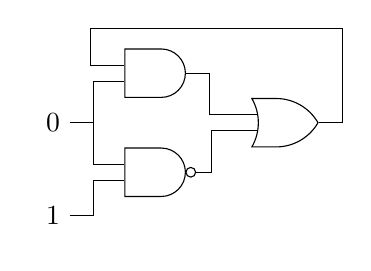
\begin{tikzpicture}[circuit logic US]
\matrix[column sep=7mm]{
& \node [and gate] (a1) {}; & \\
\node (i1) {0}; & & \node [or gate] (o) {};\\
& \node [nand gate] (a2) {}; & \\
\node (i2) {1}; & & \\
};
\draw 
(i1.east) -- ++(3mm,0) |- (a1.input 2)
(i1.east) -- ++(3mm,0) |- (a2.input 1)
(i2.east) -- ++(3mm,0) |- (a2.input 2)
(a1.output) -- ++(3mm,0) |- (o.input 1)
(a2.output) -- ++(2mm,0) |- (o.input 2)
%back-connections are problematic
(o.output) -- ++(3mm,0) -- ++(0,12mm) -- ++(-32mm,0) |- (a1.input 1)
;
\end{tikzpicture}

\end{document}
